\documentclass[conference]{IEEEtran}
\usepackage{graphicx,booktabs,tabularx,amsmath,amssymb,url,textcomp}
\usepackage[T1]{fontenc}
\graphicspath{{../}}
\hyphenation{epi-demio-logical}
\begin{document}
\title{EpiScope: A Big Data Surveillance, Forecasting and Response-Planning Platform for Seasonal, Tropical and Epidemic Diseases}
\author{\IEEEauthorblockN{Group \textbf{[number]}}
\IEEEauthorblockA{CSE 4345 Big Data Analytics, Department of Computer Science \& Engineering, Premier University, Chittagong\\
Members: \textbf{[Member 1 (ID)], [Member 2 (ID)], [Member 3 (ID)]}\\
Repository: \textbf{[URL]}\ \ Video: \textbf{[link]}}}
\maketitle
\begin{abstract}
EpiScope is a prototype national platform that turns routine health, climate and stock data into early warnings, four-week forecasts, a supply allocation plan and a preparedness calendar, behind a privacy-preserving D3.js dashboard. It is built as an Apache Spark lakehouse with idempotent incremental loads, seventeen data-quality rules, salted pseudonymisation and complementary small-cell suppression. On a synthetic national dataset with planted outbreaks (1.3 million records at scale factor 0.05), a seasonal detector finds 89\% of injected outbreaks at about one false alert per district-year; negative-binomial forecasts reduce dengue error by 36\% compared with a seasonal-naive baseline, and a linear programme with an equity floor leaves 24\% less weighted need unmet than a population-proportional split at a 60\% budget. The report states clearly which results were measured, on what hardware, and what remains for the team to verify at full scale.
\end{abstract}
\begin{IEEEkeywords}
big data, Apache Spark, disease surveillance, outbreak detection, forecasting, resource allocation, privacy, D3.js
\end{IEEEkeywords}
\section{Introduction and Problem Analysis}
Bangladesh carries a heavy and strongly seasonal burden of infectious disease. Dengue follows the monsoon, acute watery diarrhoea rises before the rains and after floods, influenza-like illness peaks in the wet season, and malaria is concentrated in the Chittagong Hill Tracts. Routine data exist, but they sit in separate systems with different formats, delays and quality, and most analysis is done afterwards in spreadsheets, so supplies often reach a district after its hospitals are already full. The brief from the Ministry of Health (a teaching case) asks for a prototype that, for every district, detects unusual rises in four disease groups, forecasts cases and hospital demand one to four weeks ahead, recommends how to allocate a limited national stock of supplies, and produces a seasonal preparedness calendar, all behind a dashboard that non-specialists can trust and that never exposes identifiable patient information.

\textbf{What we built.} EpiScope is an end-to-end Apache Spark lakehouse (bronze, silver, gold) with a seeded synthetic encounter generator tied to real geography, a rule-based quality and privacy layer, three outbreak detectors evaluated against injected ground truth, per-district negative-binomial forecasts with a rolling-origin backtest, a linear programme for supply allocation with an explicit equity floor, a seasonal calendar, and a D3.js dashboard with five coordinated views. Section~\ref{sec:cep} analyses the engineering problem, Section~\ref{sec:arch} the architecture, Sections~\ref{sec:data}--\ref{sec:eval} the methods and their evaluation, and Sections~\ref{sec:dash}--\ref{sec:limits} the dashboard, ethics and limitations. Requirement identifiers (for example ING-4, AN-5) are used throughout and mapped to files in the repository README.

\textbf{Stakeholders and needs.} The Ministry needs a defensible allocation of a fixed budget (``why did district X get more than Y?''). Surveillance epidemiologists need transparent methods and adjustable thresholds and distrust reporting artefacts treated as outbreaks. District officers need early local warnings without alert fatigue. Hospital managers need forecasts with uncertainty bands. City vector-control units need hotspots at fine resolution, and the privacy regulator requires minimal data, purpose limitation and suppression of small counts. These needs conflict, and Section~\ref{sec:cep} shows how each conflict was resolved with numbers.

\textbf{Scope and honesty about evidence.} All results in this report come from runs of the code in the repository on a single virtual CPU with 4~GB of memory, at scale factor (SF) 0.05 unless stated (about 1.3 million encounters, 5\% of the full volume), because that is the largest configuration the preparation environment could process in reasonable time. The full-scale timing at SF=1 on a 16~GB laptop has to be measured by the team; the scaling study here covers smaller factors and is clearly labelled. Real weather could not be downloaded in the preparation environment, so the weather used for the reported results is the seeded synthetic monsoon model, labelled \texttt{synthetic\_fallback} in the data; the fetch code for the Open-Meteo archive is included but was not executed there. District populations are approximate rounded values. The usability study with non-specialist users has not been performed yet and is reported as pending in Section~\ref{sec:dash}.
\section{CEP Attribute Analysis and Resolution of Conflicts}\label{sec:cep}
\subsection{Attributes P1--P7}
\textbf{P1, depth of knowledge.} The solution combines distributed storage and processing (partitioned Parquet, broadcast joins, adaptive skew handling), data integration and quality engineering, surveillance statistics (EARS, Farrington-style seasonal baselines, CUSUM), count-time-series regression with overdispersion, proper scoring rules for interval forecasts, linear optimisation with equity constraints, visual encoding and interaction design, and statistical disclosure control.
\textbf{P2, conflicting requirements.} Five explicit conflicts (C1--C5) are resolved below with experiments rather than opinion.
\textbf{P3, depth of analysis.} Detection thresholds, forecast lags, the equity floor and the aggregation level are not given by any standard; each was chosen from a threshold sweep, an ablation or a scenario grid and compared with a baseline (Section~\ref{sec:eval}).
\textbf{P4, unfamiliar issues.} Reporting delays up to 21 days (and longer after back-filling), a facility that goes silent and back-fills, duplicate submissions, cross-facility duplicate patients, invalid values, skew towards Dhaka, and changes of reporting practice. The pipeline handles each explicitly: a checksum ledger and partition merge for late data, an artefact guard in detection, quarantine with reason codes, and a patient de-duplication window.
\textbf{P5, beyond standard codes.} No standard converts forecasts into an allocation plan. We combined WHO IDSR~\cite{idsr} surveillance principles, ICD-10 coding for disease groups and data-minimisation principles with our own conversion assumptions (kept in one versioned file) and a transparent optimisation model.
\textbf{P6, stakeholders.} Section~\ref{sec:cep} lists seven stakeholder groups; role-based views, uncertainty bands and an explanation of alpha respond to their specific concerns.
\textbf{P7, interdependence.} Quality affects detection (report completeness feeds the artefact guard), forecasts and uncertainty feed demand and the optimiser, and all of them feed the dashboard. A change of the epi-week definition or a late record propagates through all stages, which is why every stage is idempotent and tested end to end.

\subsection{Conflicts}
\textbf{C1, sensitivity versus false alarms.} We swept thresholds for three detectors and plotted sensitivity against false alert episodes per district-year (Fig.~\ref{fig:det}). The operating point maximises sensitivity subject to at most one false alert episode per district-year, a limit chosen because a district officer receiving more than about one spurious alert per year would stop reading them. The result: cusum at threshold 10 detects 90\% of the injected events with 0.69 false alert episodes per district-year (Section~\ref{sec:eval}).
\textbf{C2, granularity versus privacy.} The dashboard works at district level, never at facility or patient level. Counts of one to four are suppressed everywhere, including model estimates, and suppression is complementary: if a single cell of a group is hidden while the group total is shown, the next smallest cell is hidden too, so a hidden cell cannot be recovered by subtraction. Property tests over 5000 random groups confirm that no displayed value lies between one and four and no single hidden cell is recoverable. District officers see only their own district in detail.
\textbf{C3, efficiency versus equity.} The optimiser minimises cost-weighted unmet demand subject to an equity floor $\alpha$ (every district receives at least a fraction $\alpha$ of its population share of each resource). Over five budget levels and five values of $\alpha$ we plot unmet demand against the coverage of the worst-served district (Fig.~\ref{fig:eq}). At a 60\% budget, $\alpha=0.4$ lowers the inequality of coverage (Gini) from 0.63 to 0.29 for a loss of 3.7\% in weighted unmet demand, while $\alpha=0.8$ loses 16\%; we therefore recommend the largest $\alpha$ within a 10\% loss and show the whole curve to the Ministry.
\textbf{C4, freshness versus cost.} Decisions (allocation, campaigns) are weekly, reporting delays are up to three weeks, and counts for the latest weeks are incomplete, so a daily micro-batch of the analytics is sufficient. For the first signal of the week we added a Structured Streaming path that raises a provisional alert when the count already received for the current report week exceeds the full-week threshold. In a test, 3 newly landed files (1,486 records) were processed by the streaming job in a single trigger, and the median delay between file arrival and the alert table being written was 22 seconds (maximum 22 s), well inside the five-minute target.
\textbf{C5, accuracy versus interpretability.} We use a negative-binomial regression whose coefficients officials can read (recent level, annual harmonics, rainfall and temperature lagged four to eight weeks) and compare it with the seasonal-naive baseline and with the same model without weather. For dengue the regression with weather has an MAE of 2.80 against 4.34 for the baseline and 2.97 without weather, so the readable model captures nearly all the achievable gain.
\section{Architecture and Design Decisions}\label{sec:arch}
Fig.~\ref{fig:arch} shows the architecture, which follows the reference design with the substitutions listed in Table~\ref{tab:alt}.
\begin{figure}[t]\centering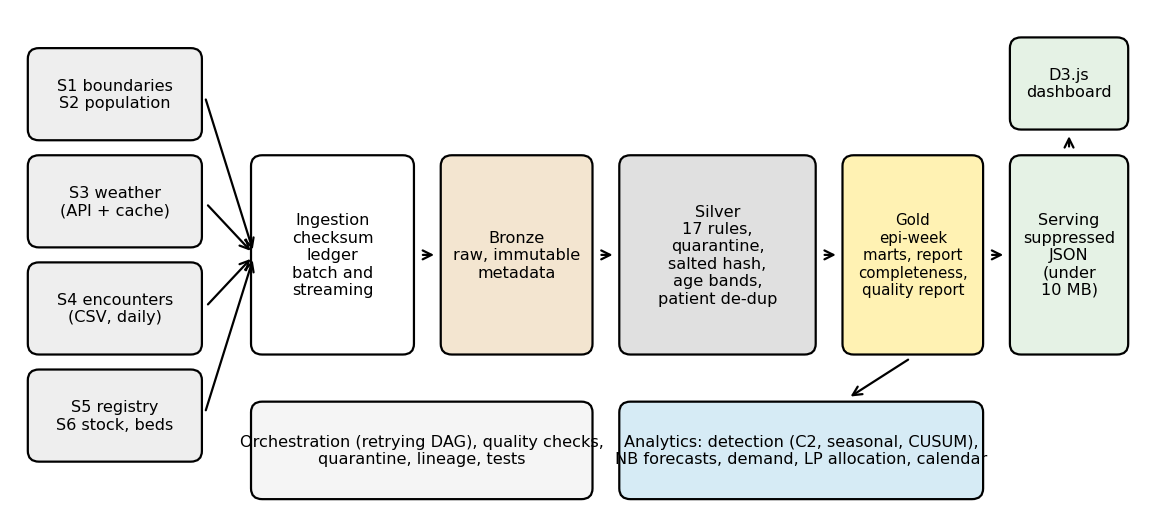
\includegraphics[width=\columnwidth]{figures/architecture.png}\caption{EpiScope architecture: sources, medallion lakehouse, analytics, suppressed serving layer and D3.js dashboard.}\label{fig:arch}\end{figure}

\textbf{Layers.} Bronze stores every landed file unmodified as strings plus \texttt{\_source}, \texttt{\_batch\_id} (first 12 hex digits of the file SHA-256), \texttt{\_file\_checksum}, \texttt{\_load\_ts}, \texttt{\_source\_file} and \texttt{\_source\_date}. Silver parses, validates against 17 rules, quarantines failures with reason codes, replaces the patient identifier by a salted SHA-256 hash, reduces age to a band, joins geography and flags cross-facility duplicate patients. Gold holds the epi-week marts: a reporting triangle (onset week by report week), weekly cases by onset week, weekly reports by report week, district report completeness, weekly weather, district stock at the end of each week, and the data-quality report. Tables are registered in the Spark SQL catalog (Hive metastore backed by Derby) under database \texttt{episcope}.

\textbf{Partitioning (ING-3).} Silver is partitioned by \texttt{epi\_year/epi\_week} of onset: almost every query is a time window, and late records (up to three weeks, longer after back-fill) touch only the most recent partitions, which can therefore be replaced with dynamic partition overwrite. Division was rejected as a partition key because eight divisions times 262 weeks would create about 2000 partitions of a few thousand rows each (the small-file problem); district is instead a column used for filtering, benefiting from Parquet min/max statistics. Gold marts use the same key. The epi-week is defined by weeks starting on Sunday and belonging to the year of their Wednesday.

\textbf{Incremental, idempotent loads (ING-4).} A ledger of file checksums makes bronze ingestion a no-op for files already loaded. Silver processes only bronze batches missing from its own ledger, computes the affected epi-weeks (plus one week either side, because a patient duplicate can straddle a week boundary), reads those existing partitions, merges, and rewrites exactly those partitions through a staging directory (Spark refuses to overwrite a path it is reading). Gold rebuilds only the weeks that silver reports as changed. A record resubmitted in a later file is rejected with reason R17 and never alters counts. An integration test loads a two-month history, re-runs it, then lands a file with three late records and one resubmission and asserts exact count changes in one epi-week.

\begin{table}[t]\caption{Design alternatives considered.}\label{tab:alt}\centering\small
\begin{tabularx}{\columnwidth}{@{}lXX@{}}\toprule
Decision & Chosen & Alternatives and reason \\\midrule
Table format & Parquet, ledger-based merge & Delta/Iceberg~\cite{delta}: time travel is attractive but adds a dependency; the reporting triangle already answers ``what did we know on date $t$'' \\
Storage & Local file system & HDFS or MinIO: not implemented; paths isolated in one module \\
Detection & EARS C2, seasonal baseline, CUSUM & Single method only: cannot show the trade-off or the artefact effect \\
Forecast model & NB GLM & Gradient boosting: possibly more accurate but harder to explain and to audit \\
Optimiser & LP with HiGHS & Integer programme: integrality adds little at this scale of units \\
Serving & Static suppressed JSON & Live API: more moving parts; JSON is adequate for weekly decisions \\
Orchestration & Python DAG with retries & Airflow: heavier than needed on a laptop \\\bottomrule
\end{tabularx}\end{table}

\textbf{Tool justification.} Spark~\cite{spark} performs every heavy transformation (ingestion, validation, joins, aggregation, grouped detection and forecasting through \texttt{applyInPandas}); pandas is used only for small reference data and final aggregated outputs. D3.js v7~\cite{d3} is the only visualisation library for the required views.
\section{Data Generation, Quality, Lineage and Privacy}\label{sec:data}
\textbf{Sources.} S1 district boundaries are the OCHA COD-AB ADM2 polygons, simplified to 120~KB for the browser. S2 populations are approximate rounded district totals entered for teaching (to be replaced by the BBS 2022 table). S3 weather comes from a fetcher for the Open-Meteo archive at district centroids with a response cache; when the cache does not cover the period the generator falls back to a seeded synthetic monsoon model and labels every row with its source. S4 encounters, S5 the registry (650 facilities: 73 hospitals, 227 upazila health complexes, 350 clinics, with beds and ICU beds) and S6 daily stock and bed snapshots are synthetic.

\textbf{Generator.} The generator is deterministic for a given seed and parameterised by the scale factor. Expected daily counts per district and disease are the product of a district share (population, urbanisation for dengue, flood exposure for diarrhoea, hill factor for malaria), an annual cycle with a district phase shift, a climate term (dengue responds to rainfall and temperature averaged over weeks 4 to 8 earlier; diarrhoea to extreme rainfall in the previous days, with a decay of about ten days) and a persistent AR(1) log-level; counts are Poisson with gamma-mixed rates, that is negative binomial, not plain Poisson. Reporting delay is right-skewed (gamma, 0 to 21 days), reports are moved off the Friday and Saturday weekend and public holidays with high probability, and a total of 34 outbreaks are injected into a separate ground-truth file: 32 local outbreaks of different size, duration and location, one slow-growing dengue outbreak and one nationwide influenza-like surge that starts in Dhaka and spreads over four weeks. One reporting artefact is injected: the largest facility of a mid-sized district goes silent for three weeks and back-fills on one day. Defects are injected at the specified rates (about 2\% resubmitted encounters, 0.5\% orphan facility keys, about 1\% invalid ages or sexes, further invalid ICD-10 codes, dates and flags) together with 1.5\% cross-facility duplicate patients. At SF=0.05 the pipeline received 1\,321\,325 records (the five-year history plus a later 14-day drop); the base volume per year is fixed at 5.0 million at SF=1, so five years give 25 million plus about 3.5\% duplicates, which is the required minimum (the volume scales linearly: SF=0.004 produced 105\,316 records, and 105\,316/0.004 is 26.3 million).

\textbf{Quality rules and quarantine (DQ-1, DQ-2).} Seventeen rules cover completeness, date validity, ordering (onset not after report), delay limit, plausible dates, age range, sex domain, ICD-10 pattern, flag domains, outcome domain, referential integrity to the registry, valid geography, and duplicates within and across loads. A row failing any rule goes to the quarantine table with all reason codes joined; nothing is silently dropped. Every load writes a report with rows in, rows quarantined and the pass rate for every rule per batch to a gold table, which the dashboard summarises. Fig.~\ref{fig:dq} shows the share of received records failing each rule. Of 1,321,325 received records, 54,112 (4.1\%) were quarantined; the largest groups were duplicate in batch (1.85\%), bad age (0.79\%), orphan facility (0.50\%), bad icd10 (0.31\%), onset after report (0.20\%). The rates match the injected defect rates (about 2\% resubmissions, 0.5\% orphan keys, 0.8\% invalid ages, 0.2\% invalid sex), which shows that the rules catch what was injected without flagging much else. Duplicates in the same load (R16) are the resubmitted records of the bulk history load; in a daily incremental load the same records are rejected as R17.
\begin{figure}[t]\centering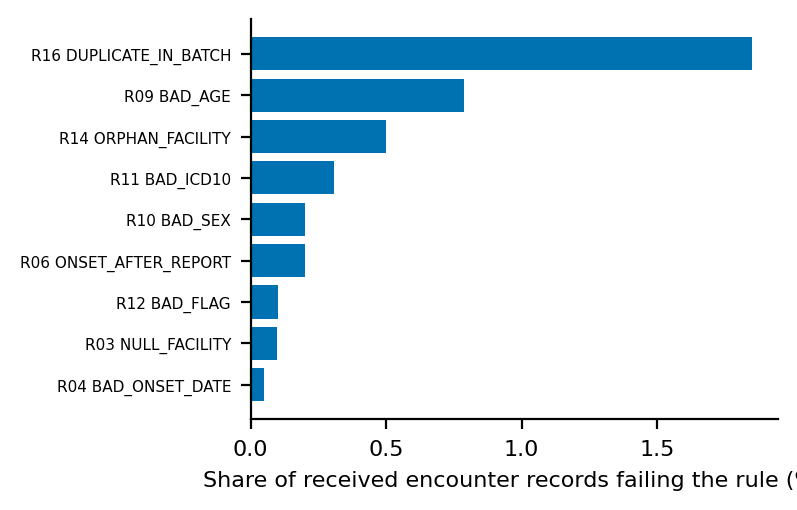
\includegraphics[width=0.78\columnwidth]{figures/quality_rules.png}\caption{Share of received encounter records failing each quality rule.}\label{fig:dq}\end{figure}

\textbf{Patient de-duplication (DQ-4).} A window over the salted patient hash and disease group flags a record as a duplicate when the previous record of the same patient has the same disease group, an onset within seven days, a different facility, the same age band and the same sex. Measured against the injected cross-facility duplicates, the window flagged 10,668 records with precision 1.000 (no false positive) and recall 0.978 against the 10,906 injected duplicates that passed validation; the missed ones are duplicates whose partner record was edited by an injected defect (for example a different sex or age band), which the compatibility test deliberately refuses to merge.

\textbf{Lineage (DQ-3).} Every gold row carries the sorted list of bronze batch identifiers that contributed to it, and the bronze ledger maps each batch to its file name, checksum and load time. \texttt{scripts/trace.py} prints the chain for any district, disease and week.

\textbf{Privacy by design (PRV-1 to PRV-3).} The raw patient identifier exists only in bronze. Silver stores SHA-256 of the salt concatenated with the identifier; the salt is read from the environment (a \texttt{.env} file created at first run with a random value and ignored by git). Exact age is converted to one of six bands and then discarded. The serving layer opens only gold tables and model outputs, never silver or bronze. Small cells (1 to 4) are suppressed with complementary suppression, and a district user receives only their own district in detail plus division-level aggregates for the rest, implemented as separate files so the restriction does not rely on the browser hiding data.
\section{Analytics Methods}\label{sec:methods}
\textbf{Detection (AN-1, AN-3).} Detection runs on counts by \emph{report} week, which is what a live system sees; counts by onset week change as late reports arrive and would hide the very artefact we want to test. Three detectors run per district and disease as a grouped \texttt{applyInPandas} job. \emph{EARS C2}~\cite{ears} compares the current week with the mean and standard deviation of eight earlier weeks separated by a two-week guard band, with the standard deviation floored at the Poisson value. The \emph{seasonal detector} (Farrington-style~\cite{farr}) builds the baseline from the same weeks $\pm3$ of up to three previous years, trims the highest 20\% of reference values so past outbreaks do not inflate it, rescales by the recent year-on-year level ratio (clipped to 0.5 to 2) and uses a quasi-Poisson dispersion. \emph{CUSUM} accumulates the standardised seasonal residuals with a reference value of 1 and a decay of 0.8 so old evidence fades. An alert also requires at least five cases.

\textbf{Reporting-artefact guard.} A facility that goes silent and then back-fills produces one week in which a large share of the district's reports are more than 14 days old. Weeks with a late share of at least 15\% and at least five late reports are flagged as artefacts, excluded from every baseline and unable to raise alerts. Facility-level silence (a facility with a trailing mean of at least three reports per week that sends none) is also computed and stored as report completeness.

\textbf{Forecasting (AN-4).} For each district, disease and horizon $h\in\{1,\dots,4\}$ a negative-binomial regression with log link predicts onset-week cases. Predictors use only data that are mature at the forecast origin, namely weeks at least four weeks old, because reports arrive up to three weeks late and a feature built from incomplete recent weeks would differ between training and use. They are the log mean of the last two mature weeks, the log mean of the last eight mature weeks, two annual harmonics, and weather: mean rainfall and temperature in the window four to eight weeks before the target week (known at the origin for $h\le4$) and the log of recent rainfall. The dispersion is estimated from a Poisson fit by the method of moments, and prediction quantiles come from the negative-binomial distribution. Series with a mean below 0.8 use an intercept and annual cycle only. All series are trained in parallel by Spark. Dengue, diarrhoea and malaria are backtested; ILI is forecast operationally for the bed-demand estimate.

\textbf{Demand conversion (AN-6).} Forecast cases over the next four weeks become resource needs with the assumptions in Table~\ref{tab:assume}: IV saline per admission (dengue 5 bags, diarrhoea 4), NS1 kits per dengue case (1.2), ORS sachets per diarrhoea case (5), antimalarial courses per malaria case (1) and length of stay for beds. District admission rates are estimated from mature weeks of the last year and shrunk towards the national rate with a prior strength of 50 cases. The upper demand sums the weekly 90\% quantiles, a deliberately conservative bound that treats weeks as perfectly correlated (the sum of quantiles is above the quantile of the sum), and the lower and mean demands are computed alike.
\begin{table}[t]\caption{Conversion assumptions (illustrative; one versioned file).}\label{tab:assume}\centering\small
\begin{tabular}{@{}lrrl@{}}\toprule Resource & Cost (USD) & Volume & Driver \\\midrule
IV saline bag & 1.20 & 1.00 & admissions \\ ORS sachet & 0.08 & 0.02 & diarrhoea cases \\
NS1 kit & 2.50 & 0.05 & dengue cases \\ Antimalarial course & 1.50 & 0.01 & malaria cases \\\bottomrule\end{tabular}\end{table}

\textbf{Allocation (AN-7, AN-8).} With districts $d$ and resources $r$, need $n_{dr}=\max(0,\hat y_{dr}-s_{dr})$ (upper demand minus stock), allocation $x_{dr}\ge0$ and unmet demand $u_{dr}\ge0$, the programme minimises $\sum w_dc_ru_{dr}$ (plus a tiny spending term that avoids pointless allocation) subject to $u_{dr}+x_{dr}\ge n_{dr}$, a national budget $\sum c_rx_{dr}\le B$, an equity floor $x_{dr}\ge\alpha p_d\sum_{d'}x_{d'r}$ and a transport limit $\sum_{d\in k}\sum_rv_rx_{dr}\le T_k$ for each division $k$. Valuing unmet demand in money makes resources comparable. The severity weight $w_d=1+(1-b_d/b_{\max})$ rises as hospital beds per 100\,000 people ($b_d$) fall. The transport limit is 1.5 times the division's population share of the national volume of need. The equity floor $\alpha$ is a policy dial: at $\alpha=0$ the model sends supplies wherever they avert the most weighted harm and may leave low-risk districts with nothing; at $\alpha=0.4$ every district is guaranteed at least 40\% of its population share of every resource, whatever its forecast. The baseline is a population-proportional split of the same budget. The programme is solved with SciPy HiGHS.

\textbf{Seasonal calendar (AN-9).} For every division and disease the weekly incidence per 100\,000 is decomposed by STL (period 52, robust). The seasonal component averaged by epi-week defines the high season as the contiguous window around the peak where it exceeds its mean by half a standard deviation; supplies should be pre-positioned six weeks and a prevention campaign started eight weeks before the season begins (stated lead-time assumptions). A season is called marked only if the seasonal strength is at least 0.3.
\section{Evaluation}\label{sec:eval}
All numbers in this section are produced by scripts in the repository from the SF=0.05 run (about 1.3 million records, seed 42, 2021--2025) unless stated. The pipeline was afterwards re-run incrementally on a separate 14-day drop (Section~\ref{sec:drop}), so the quality counts and the forecast and allocation results use the history plus those two weeks, while detection is evaluated on the history only; the machine was one virtual CPU with 4~GB of memory.

\subsection{Outbreak detection (AN-2, AN-3)}
Detection is scored against the ground-truth file, which the detection code never reads. The first 14 months provide baseline history for the seasonal detector, so all methods are evaluated on the common period starting 2022-01-16, which contains 92 injected outbreak events (district by disease; the nationwide surge counts once per district). An event is detected if an alert episode overlaps the outbreak window extended by one week; an alert episode with no overlap with any true outbreak of the same district and disease (tolerance one week before and two after) is a false alert; the false alert rate is episodes per district-year over all diseases. Table~\ref{tab:det} gives the best admissible threshold of each method under the limit of one false alert episode per district-year, and Fig.~\ref{fig:det} shows the full trade-off.
\begin{table}[t]\caption{Detection at the best admissible threshold. Local: sensitivity for local outbreaks only. FA/yr: false alert episodes per district-year. Days: median days to detection.}\label{tab:det}\centering\small
\begin{tabular}{@{}lrrrrr@{}}\toprule Method & Thr. & Sens. & Local & FA/yr & Days \\\midrule
EARS C2 & 8 & 53\% & 50\% & 0.74 & 21 \\
Seasonal (Farrington-style) & 6 & 89\% & 79\% & 0.98 & 20 \\
CUSUM, seasonal & 10 & 90\% & 79\% & 0.69 & 28 \\
\bottomrule\end{tabular}\end{table}
\begin{figure}[t]\centering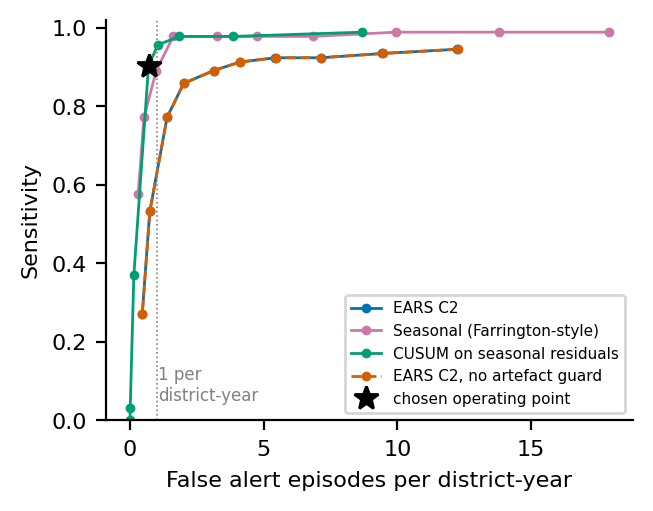
\includegraphics[width=0.9\columnwidth]{figures/detection_tradeoff.png}\caption{Detection trade-off (conflict C1): sensitivity against false alert episodes per district-year for threshold sweeps. The star marks the operating point.}\label{fig:det}\end{figure}
The method chosen by the rule is CUSUM, seasonal at threshold 10 (90\% of events detected, 0.69 false alert episodes per district-year, median 28 days from outbreak start to the end of the first alerting report week). The comparison shows what the seasonal baseline buys: EARS C2 with its eight-week baseline most likely mistakes the steep monsoon rise of dengue for outbreaks (we did not separate false alerts by cause), so it needs a threshold of 8 to stay under one false alert per district-year and then detects only 53\% of events, whereas the seasonal detector detects 89\% at a similar false alert rate (0.98 per district-year at threshold 6). Detection is slow in absolute terms (about three to four weeks) because the injected outbreaks ramp up gradually and alerts are raised at the end of a report week. \textbf{Reporting artefact.} In the district of the silent facility, with back-fill on 2024-07-29, a detector without the guard raised alerts in 1 week(s) around the back-fill, while the guarded pipeline raised 0; the guard flagged 4 report week(s) as artefacts. The slow-growing dengue outbreak and the nationwide surge are included in the event counts above.

\subsection{Forecasting backtest (AN-5)}
The rolling-origin backtest covers the last 52 forecastable origins for dengue, diarrhoeal disease and malaria (64 districts, four horizons, 119\,808 forecast rows per model family), refitting every four origins and using only data mature at each origin. Targets are final onset-week counts. Table~\ref{tab:fc} reports the mean absolute error (MAE), the 80\% and 95\% prediction interval coverage and the weighted interval score (WIS~\cite{bracher}, with a median and 80\% and 95\% intervals) for the regression with weather, the same regression without weather, and the seasonal-naive baseline (the count of the same week one year earlier, with intervals from the same dispersion).
\begin{table*}[t]\caption{Rolling-origin backtest, 52 origins, horizons 1 to 4, all 64 districts. Mean observed weekly counts per district: dengue 8.2, diarrhoea 15.7, malaria 2.4.}\label{tab:fc}\centering\small
\begin{tabular}{@{}llrrrrr@{}}\toprule Disease & Model & MAE & MAE/mean & WIS & 80\% cov. & 95\% cov. \\\midrule
dengue & NB regression with weather & 2.80 & 0.34 & 1.32 & 89\% & 97\% \\
 & NB regression, no weather & 2.97 & 0.36 & 1.45 & 89\% & 97\% \\
 & Seasonal naive & 4.34 & 0.53 & 2.17 & 77\% & 88\% \\
\midrule
diarrhoea & NB regression with weather & 7.53 & 0.48 & 3.57 & 85\% & 95\% \\
 & NB regression, no weather & 7.61 & 0.49 & 3.56 & 88\% & 96\% \\
 & Seasonal naive & 9.82 & 0.63 & 4.79 & 76\% & 88\% \\
\midrule
malaria & NB regression with weather & 1.12 & 0.47 & 0.51 & 93\% & 98\% \\
 & NB regression, no weather & 1.13 & 0.48 & 0.51 & 93\% & 98\% \\
 & Seasonal naive & 1.52 & 0.64 & 0.70 & 90\% & 96\% \\
\bottomrule\end{tabular}\end{table*}
The regression reduces MAE relative to the seasonal-naive baseline by 36\% for dengue, 23\% for diarrhoea and 27\% for malaria, and it beats the baseline in 98\%, 86\% and 100\% of districts respectively. The weather covariates matter little: relative to the same model without weather the MAE improves by 5.7\% for dengue, 1.0\% for diarrhoea and 1.6\% for malaria. This is expected for horizons of one to four weeks, where recent counts and the annual cycle carry most of the information; weather lagged four to eight weeks would be expected to matter more at longer horizons, which we did not test and the brief does not require. Because the generator itself links dengue to lagged weather, this gain may overstate what real data would show. Interval coverage is conservative: the 80\% intervals cover 89\% of dengue observations and 85\% for diarrhoea, above the nominal level, probably because the dispersion estimated from the training pairs also absorbs the injected outbreaks (we did not test this explanation); the baseline's intervals under-cover (77\%). For hospital managers an interval that is slightly too wide is the safer error. The error relative to the mean count is nearly flat across horizons for dengue (0.34 at one week, 0.34 at four; Fig.~\ref{fig:fc}). This is plausible because the predictors are anchored on weeks at least four weeks old, so even horizon one is an effective five-week-ahead forecast; the cost is that the most recent weeks are not used, which nowcasting would fix (future work). The mean cases per district-week are small (single digits to a few tens), so relative errors of 30\% or more are the realistic range; the point is that the intervals are honest. \textbf{Interpretability (C5).} Because the weather model is only slightly better than its no-weather version and far better than the baseline, and because both are readable regressions, we kept the regression and did not add a black-box model; a gradient-boosted model would have to beat these numbers clearly to justify losing the ability to explain each forecast to an official.
\begin{figure*}[t]\centering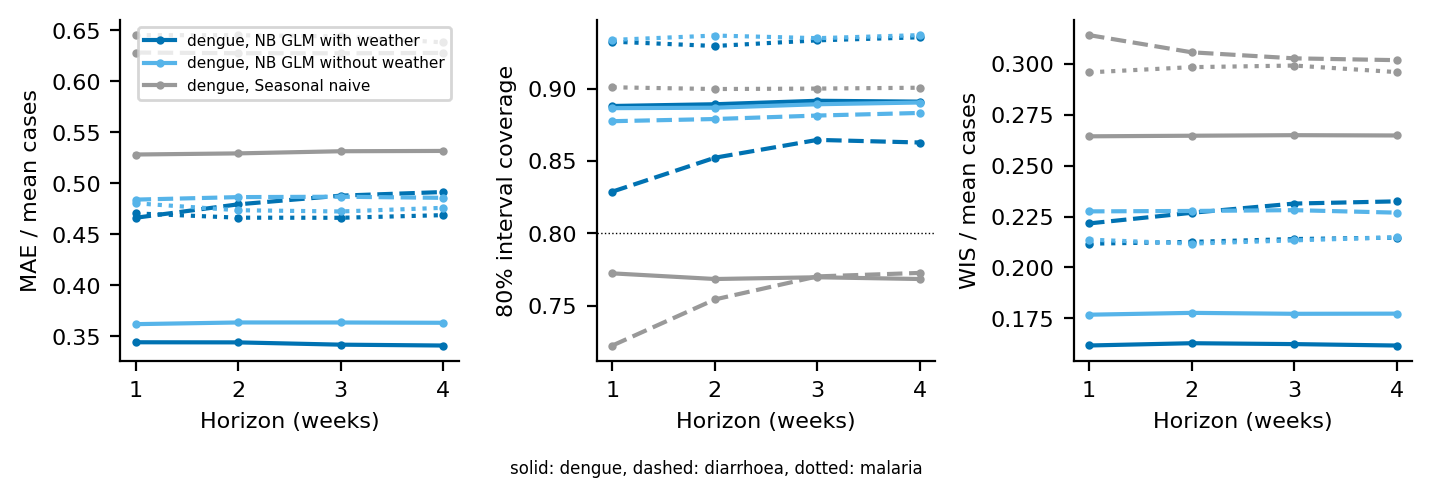
\includegraphics[width=\textwidth]{figures/forecast_backtest.png}\caption{Backtest by horizon: error relative to the mean observed count, 80\% interval coverage (dotted line is the nominal 80\%) and weighted interval score.}\label{fig:fc}\end{figure*}

\subsection{Allocation against the baseline (AN-7, AN-8)}
The planning scenario uses the forecast issued at the origin with the largest national need, the week of 2025-08-24, near the dengue peak; at the latest origin (2026-01-04, low season) the national need is only USD 281, against USD 40\,478 at the peak, so an allocation study there would be trivial. Stocks are those on hand at the origin week. Table~\ref{tab:alloc} compares the optimiser with the population-proportional split at a 60\% budget, and Fig.~\ref{fig:eq} shows the efficiency--equity curves for all five budgets.
\begin{table}[t]\caption{Allocation at a 60\% budget (thousand USD of weighted unmet demand). Waste: allocation above need caused by the floor. Loss: increase in unmet demand over $\alpha=0$.}\label{tab:alloc}\centering\small
\begin{tabular}{@{}lrrrrr@{}}\toprule $\alpha$ & Unmet & vs base & Gini & Waste & Loss \\\midrule
0 & 27.8 & 23.7\% & 0.63 & 0.0 & 0.0\% \\
0.2 & 28.3 & 22.4\% & 0.41 & 0.2 & 1.7\% \\
0.4 & 28.9 & 20.9\% & 0.29 & 0.4 & 3.7\% \\
0.6 & 30.2 & 17.3\% & 0.23 & 1.1 & 8.4\% \\
0.8 & 32.2 & 11.7\% & 0.19 & 2.2 & 15.8\% \\
pop. baseline & 36.5 & --- & 0.20 & --- & --- \\
\bottomrule\end{tabular}\end{table}
\begin{figure*}[t]\centering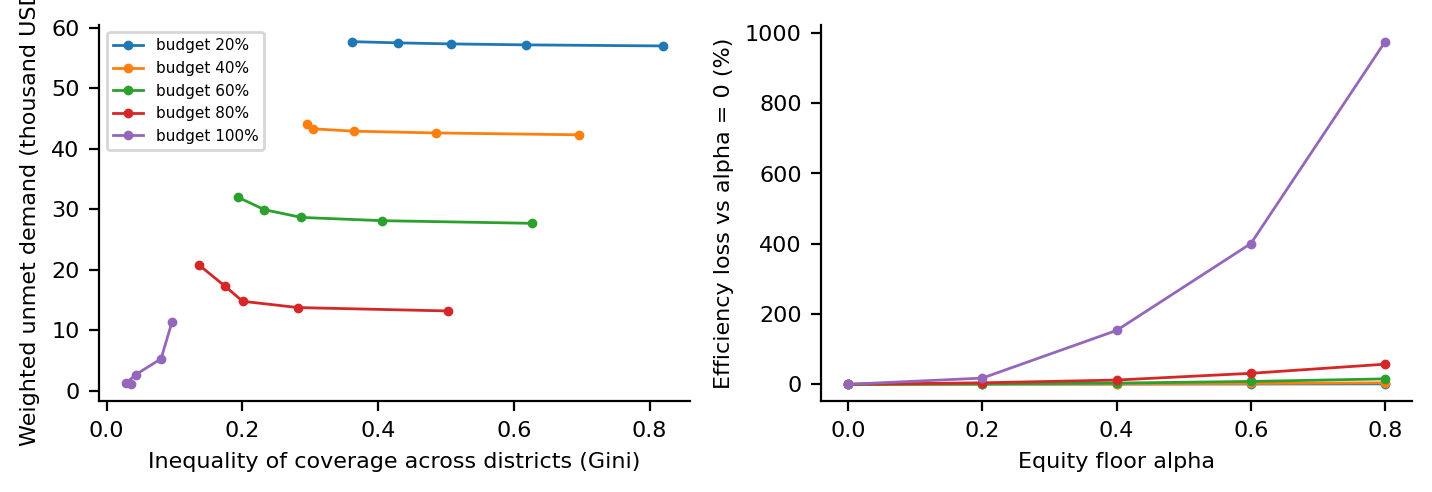
\includegraphics[width=0.8\textwidth]{figures/efficiency_equity.png}\caption{Efficiency--equity trade-off (conflict C3). Left: weighted unmet demand against inequality of coverage for $\alpha\in\{0,0.2,0.4,0.6,0.8\}$ (points along each line, left to right is more equal) and five budgets. Right: efficiency loss relative to $\alpha=0$.}\label{fig:eq}\end{figure*}
At a 60\% budget the optimiser with no equity floor cuts weighted unmet demand by 24\% relative to the population-proportional split (3\% at 20\%, 52\% at 80\% and 95\% at a full budget). In this data need is concentrated by construction: dengue demand follows the large cities while stock follows hospital beds, so a proportional rule sends supplies to districts that do not need them. The cost of equity is small at moderate floors and large at high ones: $\alpha=0.4$ costs 3.7\% of weighted unmet demand and reduces the Gini coefficient of coverage across districts from 0.63 to 0.29, while $\alpha=0.8$ costs 16\% and wastes USD 2.2 thousand on allocation above need. The worst-served district gets almost nothing at every budget below 100\% (its coverage stays near zero whatever $\alpha$), because the equity floor guarantees a share of the \emph{national} allocation in proportion to population, not a share of local need; the Gini coefficient and the efficiency loss are therefore the informative measures, and a minimum-coverage guarantee would need a different constraint (future work). \textbf{Recommended policy.} Choosing the largest $\alpha$ whose loss is within 10\% of the unconstrained optimum gives $\alpha=0.8$ at a 20\% budget, 0.8 at 40\%, 0.6 at 60\%, 0.2 at 80\% and 0 at 100\% (at a full budget unmet demand is almost zero without a floor, so any floor looks expensive in relative terms). This answers the Ministry's question: a district receives more than another because its forecast upper demand minus stock is larger, weighted by how few hospital beds it has per head, and every district receives at least $\alpha$ times its population share.

\subsection{Scalability and Spark optimisations (ENG-2, ENG-3)}
\begin{table}[t]\caption{Runtime by stage (seconds) at three scale factors on one virtual CPU, 4~GB memory. Rows = encounter records generated.}\label{tab:scale}\centering\footnotesize
\begin{tabular}{@{}rrrrrrrr@{}}\toprule SF & Rows & Gen. & Bronze & Silver & Gold & Detect & Total \\\midrule
0.01 & 262\,930 & 16 & 223 & 179 & 202 & 66 & 687 \\
0.025 & 656\,626 & 24 & 266 & 203 & 204 & 71 & 768 \\
0.05 & 1\,314\,392 & 36 & 219 & 204 & 180 & 56 & 695 \\
\bottomrule\end{tabular}\end{table}
Between scale factors 0.01 and 0.05 the data grew 5.0-fold (262,930 to 1,314,392 records) but the total time of the data stages stayed almost constant (687 s to 695 s). At these sizes the cost is therefore dominated by fixed overheads, chiefly Spark start-up per stage and reading 1826 small daily encounter files and 1826 stock files (bronze takes about 220 s at every scale), not by data volume. The experiment shows that the pipeline does not slow down for 1.3 million records; it does \emph{not} show how it scales to 25 million, and no extrapolation to SF=1 is made. The forecasting stage (634 s at SF=0.05) does not depend on the number of rows: it trains models per district, disease and horizon on weekly series, so its cost is set by the number of series (about 200) and the length of history. \textbf{The required runs at SF=0.25, 0.5 and 1 were not performed}: the preparation environment could not hold that volume in reasonable time. The team must run \texttt{make scaling} on a 16~GB laptop, replace this table and state the machine; the target is 45 minutes at SF=1.
\begin{table}[t]\caption{Spark optimisations, median of three runs on 1.26 million silver records. Spark REST-API metrics are in \texttt{docs/spark\_optimisations.json}.}\label{tab:opt}\centering\footnotesize
\begin{tabularx}{\columnwidth}{@{}Xrrr@{}}\toprule Optimisation & Before (s) & After (s) & Speed-up \\\midrule
Broadcast join of the 650-row registry & 5.78 & 2.26 & 2.6$\times$ \\
Compaction of 200 files to 4 & 1.12 & 0.45 & 2.5$\times$ \\
Adaptive query execution on a skewed aggregation & 6.46 & 3.17 & 2.03$\times$ \\
Key salting (8 salts) & 6.46 & 4.57 & 1.41$\times$ \\
Partition pruning, path read & 0.52 & 3.58 & 0.14$\times$ \\
Partition pruning, catalog table & 0.52 & 0.73 & 0.71$\times$ \\
\bottomrule\end{tabularx}\end{table}
\textbf{Broadcast join.} Enriching encounters with the facility registry by a sort-merge join shuffles every encounter by facility; broadcasting the 650-row registry removes that shuffle and is 2.6 times faster. The hint changes the physical plan from a sort-merge join to a broadcast hash join (to be confirmed in the Spark UI). \textbf{Compaction.} Writing with 200 partitions produced 200 small files; compacting to 4 cuts a column scan from 1.12 to 0.45 s (2.5 times) because task scheduling and footer reads dominate small files; the silver and gold writers therefore repartition by the partition key before writing. \textbf{Skew.} The largest district (BD3026) holds 126,237 of 1,260,773 records, about 10\%, which is far milder than a power-law skew; adaptive query execution gave a 2.03-fold gain, whereas manual salting did not help (1.41-fold) because the extra aggregation stage costs as much as the imbalance it removes. We report this negative result rather than claim a gain: at 10\% skew AQE is sufficient. \textbf{Partition pruning.} Pruning reduced the input partitions of a one-week query from 9 to 1, yet at this size it did not make the query faster: reading the path pays for listing 262 partition directories and the unpartitioned copy benefits from Parquet min/max statistics on a 108~MB table (the catalog comparison gives 0.73 s partitioned against 0.52 s unpartitioned). We keep the layout because it is what lets late data replace only the affected weeks, and its read benefit would appear at the 25-million-record scale, which we could not test. Spark UI screenshots must be taken by the team (instructions in \texttt{docs/TEAM\_TODO.md}); the stage counts, shuffle bytes and task counts from the REST API of the same runs are stored in the JSON file.

\subsection{Streaming path (ING-6) and tests (ENG-4)}
\textbf{Streaming.} The Structured Streaming job reads new encounter files from a landing directory, validates and pseudonymises them with the same rules as the batch path, and maintains live counts per district, disease and report week. In a test with 3 freshly copied files (1,486 records) it produced 147 live count rows, of which 0 were provisional alerts, with a median latency from file arrival to alert table of 22 s and a maximum of 22 s on one virtual CPU, within the five-minute requirement. The latency includes Spark job start-up because the test used a run-once trigger; a continuously running job would be faster.
\textbf{Tests.} The test suite (\texttt{make test}) result was: \emph{14 passed in 489.60s (0:08:09)}. It covers each quality rule firing on a crafted bad row, salted hashing and the absence of direct identifiers in silver, the optimiser constraints (budget, equity floor, non-negativity, transport) and optimality against the baseline, suppression properties, epi-week arithmetic against Spark, and an integration test that loads a two-month history twice, then lands a late record file and a resubmission and asserts exact count changes in a single epi-week.
\subsection{Hidden-drop rehearsal and idempotency}\label{sec:drop}
We generated a separate 14-day drop (seed 99, 1--14 January 2026, same schema, about 6\,900 reported records, four new outbreaks, a silent facility, doubled defect rates and late reports for earlier weeks) and ran \texttt{make incremental} without changing any code. The run finished in about 16 minutes on one CPU, of which the forecasting stage is most. Silver grew from 1\,260\,773 to 1\,267\,213 records, the quarantine from 53\,619 to 54\,112 rows and the total of gold cases from 1\,250\,126 to 1\,256\,545. Running the same command again changed nothing: all four counts were identical, silver contained no duplicate encounter identifier, and the runner stopped after the gold stage because no new epi-week had been rebuilt (112 s, mostly Spark start-up). This is the behaviour required for the instructor's hidden drop; the drop files were produced by our own generator, so compatibility with another generator rests on the schema contract and the alias handling for stock field names.
\section{Dashboard Design Rationale and Usability}\label{sec:dash}
The dashboard (D3.js v7, no other charting library) is built for decision-makers who are not data scientists. Each view answers one question and all views share one state object, so selecting a district, a disease or a time range in any view filters or highlights all others (Fig.~\ref{fig:dash}).
\begin{figure*}[t]\centering
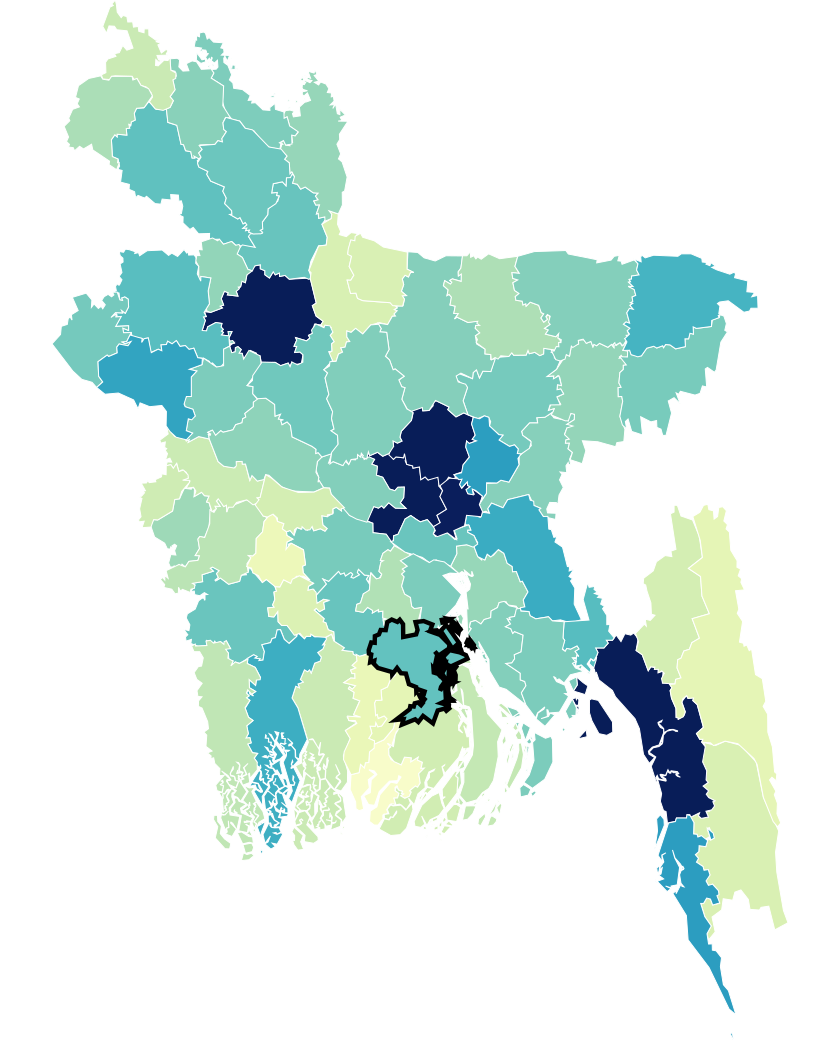
\includegraphics[width=0.30\textwidth]{figures/dash_map.png}\hfill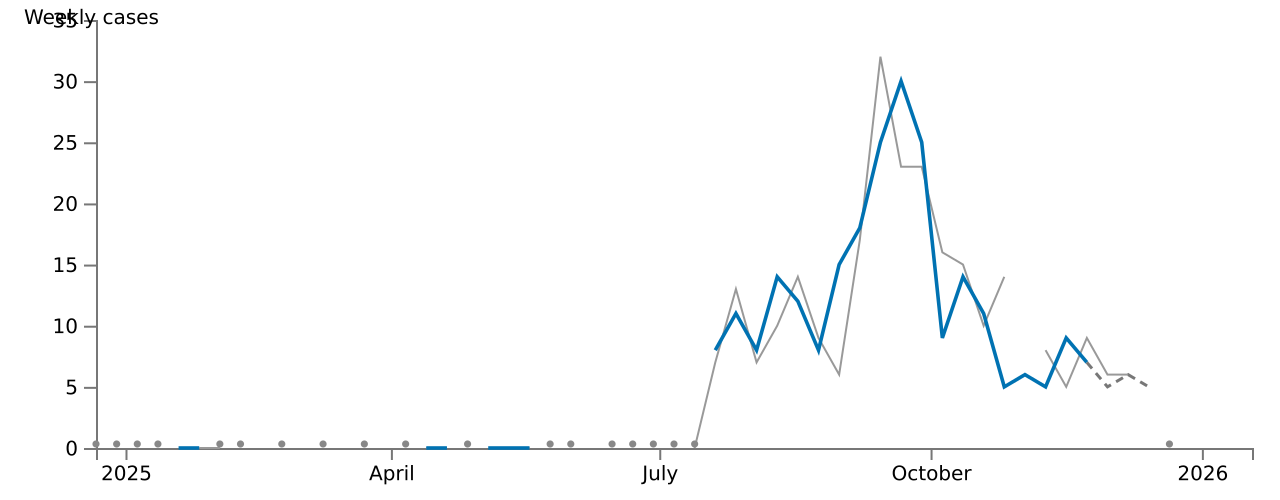
\includegraphics[width=0.66\textwidth]{figures/dash_ts.png}\\[2pt]
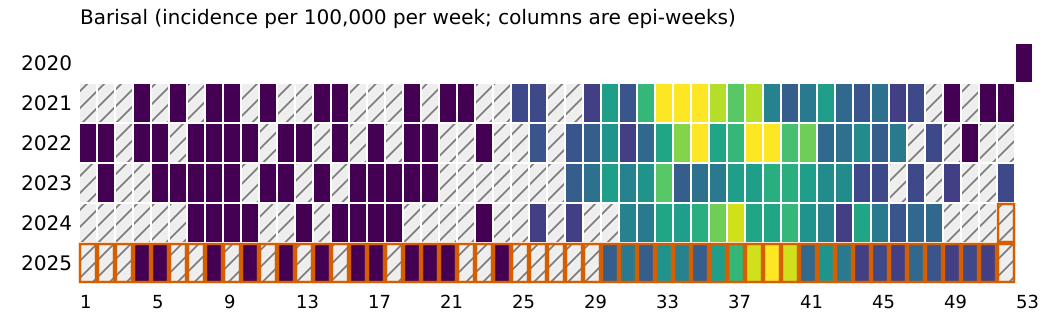
\includegraphics[width=0.48\textwidth]{figures/dash_heat.png}\hfill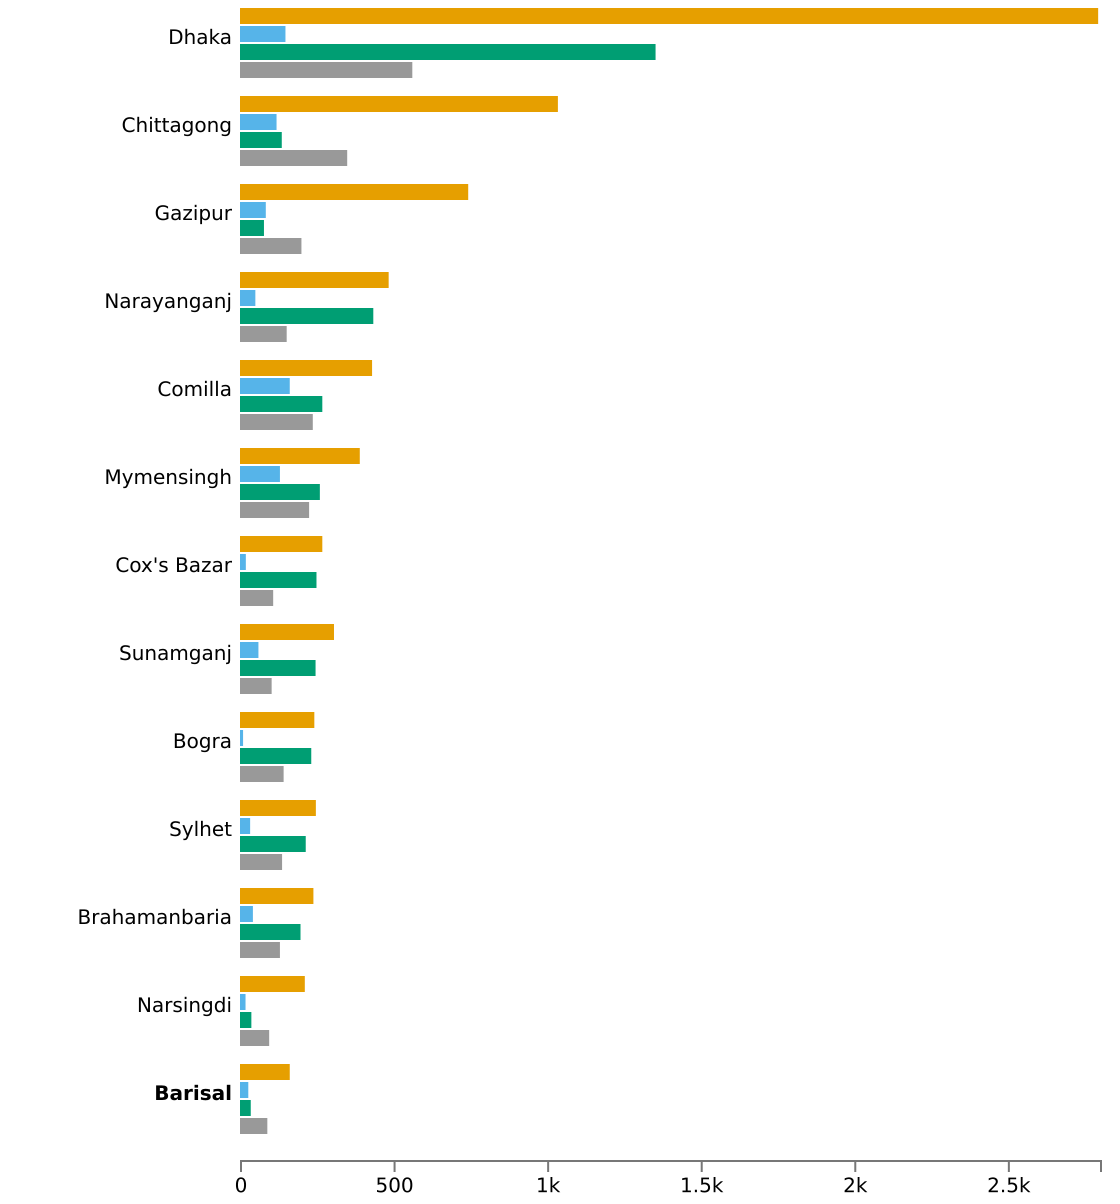
\includegraphics[width=0.48\textwidth]{figures/dash_alloc.png}
\caption{Views 1 to 4 rendered from the dashboard code on the exported data (jsdom rendering, no browser available in the build environment). Top: incidence map with the selected district outlined, and the time series for that district (blue: cases by onset week; grey: cases as reported; dashed tail: weeks with late reports pending; grey dots: suppressed weeks). Bottom: seasonal heatmap by year and epi-week, and demand, stock and recommended allocation.}\label{fig:dash}\end{figure*}

\textbf{The five required views.} (1) A district choropleth of incidence per 100\,000 for the brushed time range, with triangular markers for districts in alert and hatching for suppressed values. (2) A time series for the selected district (or the whole country) with cases by onset week, cases as reported (the basis of alerts), the 80\% forecast band for the next four weeks, the alert threshold line and alert markers; a brush on the context chart sets the time range for every view. (3) A seasonal heatmap, either year by epi-week for the selected district or all districts by epi-week. (4) An allocation view comparing forecast upper demand, current stock, recommended allocation and the population-proportional baseline for a chosen resource. (5) A ranked early-warning table of districts by alert score, with reported cases, alert status, four-week forecast and bed gap. Beyond the required views the page has a data-quality panel, the seasonal preparedness calendar, and a what-if panel.

\textbf{What-if panel (VIS-5).} Sliders set the budget, the equity floor and the detection threshold. Allocations come from a precomputed grid of 25 scenarios (five budgets times five values of $\alpha$), and alerts are recomputed in the browser from the stored scores, so no server is needed. Two small charts show where the current setting sits on the efficiency--equity curve and on the detection trade-off curve, which lets a user see what a change costs before making it.

\textbf{Scale-aware design (VIS-4).} The browser loads only aggregated, suppressed JSON: 1.7~MB for the national bundle (3.9~MB for all files including the 64 district files, against the 10~MB limit); never line-level data. The national bundle holds district by disease by week counts (64 districts by 4 diseases by about 260 weeks), detection scores for the last 104 weeks, the four-week forecasts and the allocation grid. A district officer's browser loads a division-level file (aggregates only) and the file of their own district. Aggregation to districts and weeks was chosen because it is the finest level at which most cells exceed the suppression limit (Section~\ref{sec:cep}) and the level at which decisions are made.

\textbf{Honest design (VIS-6).} Palettes are colour-blind safe (ColorBrewer YlGnBu, viridis and the Okabe--Ito set), every symbol is also coded by shape or pattern (triangles for alerts, hatching for suppressed cells), forecasts are never shown without their band, weeks whose counts are still incomplete are drawn dashed and labelled, and every panel carries the data-freshness stamp (latest report date, build time, forecast origin).

\textbf{Verification.} A headless test loads the dashboard in jsdom against the exported data, checks that all views draw (64 districts, ranking rows, heatmap cells, allocation bars, what-if charts, calendar), exercises linked selection, all diseases, all three alert methods, both heatmap layouts, brushing, the what-if sliders and the district-officer role, and fails on any script error. It passes. It cannot judge legibility or layout in a real browser.

\textbf{Usability study.} The assignment requires a check with at least two non-computer-science users. It has not been carried out yet, so this report makes no usability claim. The protocol (five tasks: find the district with the highest dengue alert, read the forecast direction and its uncertainty, find the recommended IV saline for a district at a 60\% budget, explain a hatched cell, and describe what changes in the district-officer view) and the record sheet are in \texttt{docs/TEAM\_TODO.md}. The team must run it with at least two non-specialist users, record success and time per task, fix what confuses them, and replace this paragraph with the findings.
\section{Ethical, Societal and Sustainability Considerations}\label{sec:ethics}
\textbf{Privacy and re-identification.} Health records are among the most sensitive data a state holds. The design limits risk at four points: identifiers are hashed with a secret salt at the bronze-silver boundary and exact age is discarded; the dashboard receives only aggregates; counts of one to four are suppressed with complementary suppression; and a district role cannot download other districts' detail because that detail is not in its files. Residual risks remain. A hashed identifier is still a pseudonym, so silver must stay inside the secure zone. Weekly district counts of five or more can still be linked with outside knowledge in very small districts, and repeated releases can be differenced. A public release would need formal protection such as differential privacy: adding calibrated noise to weekly counts (a Laplace mechanism with sensitivity one per person and a privacy budget split across the 261 weeks and 256 series, a large total) would make small-district series very noisy, which is why we do not claim it for public release and keep the dashboard restricted to authorised officials. A k-anonymity check~\cite{sweeney} on record-level extracts (PRV-4) was not implemented because the system never produces such extracts.

\textbf{Equity and misuse.} Allocation rules embed value judgements. Weighting unmet demand by hospital beds per capita directs scarce supplies to under-resourced districts, but an unconstrained optimiser can leave low-risk districts with nothing; the equity floor makes the trade-off explicit and the dashboard shows what each level of $\alpha$ costs in efficiency and what it buys in coverage of the worst-served district. Forecast error is not uniform: sparse districts (hill districts with few cases) have wide intervals, so a rule that favours high-count districts would systematically under-serve them. Alerts can stigmatise a district or community; the dashboard therefore shows alert status for officials only and avoids naming facilities. Models and thresholds could be misused to justify cutting support to districts with ``low'' forecasts; the policy brief states the limits of the forecasts.

\textbf{Sustainability and cost.} The platform runs on a laptop and a modest server, uses open-source software, and relies on columnar compression and partition pruning to avoid scanning unnecessary data. Precomputed scenario grids avoid running an optimisation server. A national deployment would need sustained funding for data quality at facility level, which matters more than model sophistication: the largest source of error in any surveillance system is missing or late reporting.

\textbf{AI assistance and authorship.} AI coding assistance was used and is documented in \texttt{AI\_USAGE.md}. Every member is responsible for being able to explain the code they present.
\section{Limitations and Future Work}\label{sec:limits}
\textbf{Synthetic data.} Every quantitative result describes behaviour on data generated by our own process, the situation against which the ``parable of Google Flu''~\cite{lazer} warns. Detection sensitivity depends on the size and shape of the injected outbreaks; forecast skill depends on how strongly the generator ties dengue to lagged weather, and the weather-model advantage in particular is built in by construction. Results on real DHIS2 data would be less favourable. The weather used for the reported results is synthetic (Open-Meteo could not be reached from the preparation environment); the fetch code is untested against the live API. Populations are approximate.

\textbf{Scale.} The reported runs use SF=0.05 on one virtual CPU; scaling beyond is extrapolated or must be measured on the team's laptop (SF=1, 25 million records). Spark was used in local mode; behaviour on a real cluster was not tested.

\textbf{Not implemented.} HDFS or an object store (ING-5), Delta Lake or Iceberg with time travel (ING-7), a k-anonymity check and differential privacy prototype (PRV-4, discussed only), the SEIR scenario module (AN-10), and the mobile or playback dashboard view (VIS-7). Weather in the forecast is not itself forecast: horizons up to four weeks use only observed weather four or more weeks old, which avoids the problem but limits the benefit.

\textbf{Methodological.} Forecast intervals ignore parameter uncertainty and so tend to be too narrow for series with little data; demand upper bounds sum weekly quantiles and are conservative; alert episodes and false-alert counts depend on the definition of an episode and a tolerance window around each true outbreak. The artefact guard handles one kind of artefact (back-fill after silence); a change of case definition would need a different guard. The usability study with non-specialist users is pending.

\textbf{Future work.} Nowcasting of the incomplete recent weeks from the reporting triangle (a moving-average completion factor would let horizon one use the last four weeks); an ensemble that adds a gradient-boosted model for accuracy while keeping the GLM as the audited reference; integer programmes with lead times and multiple periods; streaming alerts at daily resolution; and real data through a DHIS2 connector with the same bronze contract.

\begin{thebibliography}{10}
\bibitem{ears} L.~Hutwagner, W.~Thompson, G.~M. Seeman, T.~Treadwell, ``The bioterrorism preparedness and response Early Aberration Reporting System (EARS),'' \emph{J. Urban Health}, vol.~80, no.~1, 2003.
\bibitem{farr} C.~P. Farrington, N.~J. Andrews, A.~D. Beale, M.~A. Catchpole, ``A statistical algorithm for the early detection of outbreaks of infectious disease,'' \emph{J. R. Stat. Soc. A}, vol.~159, no.~3, 1996.
\bibitem{bracher} J.~Bracher, E.~L. Ray, T.~Gneiting, N.~G. Reich, ``Evaluating epidemic forecasts in an interval format,'' \emph{PLoS Comput. Biol.}, vol.~17, no.~2, 2021.
\bibitem{lazer} D.~Lazer, R.~Kennedy, G.~King, A.~Vespignani, ``The parable of Google Flu: traps in big data analysis,'' \emph{Science}, vol.~343, no.~6176, 2014.
\bibitem{spark} M.~Zaharia \emph{et al.}, ``Apache Spark: a unified engine for big data processing,'' \emph{Commun. ACM}, vol.~59, no.~11, 2016.
\bibitem{delta} M.~Armbrust \emph{et al.}, ``Delta Lake: high-performance ACID table storage over cloud object stores,'' \emph{PVLDB}, vol.~13, no.~12, 2020.
\bibitem{d3} M.~Bostock, V.~Ogievetsky, J.~Heer, ``D3: Data-Driven Documents,'' \emph{IEEE TVCG}, vol.~17, no.~12, 2011.
\bibitem{sweeney} L.~Sweeney, ``k-anonymity: a model for protecting privacy,'' \emph{Int. J. Uncertainty, Fuzziness Knowl.-Based Syst.}, vol.~10, no.~5, 2002.
\bibitem{idsr} World Health Organization, \emph{Technical Guidelines for Integrated Disease Surveillance and Response in the African Region}, 3rd ed.
\end{thebibliography}

\appendices
\section{Policy Brief for the Director, Disease Control and Preparedness Unit}\label{app:brief}
\textbf{Purpose.} EpiScope is a working prototype that uses routine reports, weather and stock records to warn of rising disease, forecast hospital demand for the next four weeks and suggest where to send limited supplies. The numbers below come from a trial on synthetic data with known, planted outbreaks; they show how the system behaves, not what is happening in the country.

\textbf{1. Current situation.} In the trial year the dengue season built up from July and peaked in September. At the planning week of 2025-08-24, just before the peak, the supplies needed for the next four weeks exceeded what the districts held by about USD 40\,478 for the four items we track (IV saline, oral rehydration salts, dengue test kits and malaria medicine). By the latest week (2026-01-04, low season) the shortfall was only about USD 281. Large cities need the most, while stocks follow hospital size, so shortages appear in a few districts first.

\textbf{2. Three recommendations and their expected effect.}
\begin{enumerate}
\item \textbf{Send supplies by forecast need, not by population.} With 60\% of the national need funded, a forecast-based allocation leaves 24\% less urgent need unmet than a population-proportional split; with 80\% funded the gain is 52\%. The gain is largest when money is tight but not absent.
\item \textbf{Keep a guaranteed minimum for every district.} Giving each district at least 40\% of its population share of every item costs 3.7\% in overall effectiveness at a 60\% budget and cuts the inequality of coverage between districts from 0.63 to 0.29 (a lower figure is fairer). Raising the guarantee above about 60\% starts to waste supplies. The Ministry should decide this value as a policy choice; the dashboard shows the cost of each setting.
\item \textbf{Prepare by season and act on early warnings.} Begin pre-positioning stock six weeks, and prevention campaigns eight weeks, before the high season of each division (for dengue: season starts between weeks 30 and 32 depending on the division, and ends between weeks 42 and 44, in epidemiological weeks). The warning system found 89\% of the planted outbreaks with about 1.0 false alarm per district per year, typically 20 days after the outbreak began, so a warning should trigger a check and local response, not a final decision.
\end{enumerate}

\textbf{3. How to read the dashboard.} The map shows cases per 100\,000 people for the weeks selected on the small time bar below the line chart; a triangle marks a district with an active warning. Click a district to see its weekly cases, the forecast for the next four weeks (the shaded band is the range in which about four out of five outcomes are expected) and, below, supplies needed, held and recommended. A hatched or blank cell means the number is too small to be shown to protect privacy. A dashed line at the end of a series means late reports are still arriving and the count will rise. Use the sliders on the right to see how the plan changes with the budget and with the minimum guarantee.

\textbf{4. Confidence and limitations.} The forecast is more accurate than simply repeating last year (about 36\% lower error for dengue) but weekly counts in small districts are uncertain, and the bands are deliberately wide. The trial used synthetic data, approximate populations and simulated weather; accuracy on real data will be lower. Warnings come about three to four weeks after an outbreak starts because reports arrive late. The supply conversion factors (for example bags of saline per admission) are assumptions to be replaced by national protocols. The system supports decisions; it does not replace the judgement of district and national officers.

\textbf{5. Data-protection assurance.} Patient identities are scrambled with a secret key the moment records enter the system and never reach the dashboard. The dashboard shows only totals by district and week; counts of one to four are hidden, and hidden numbers cannot be worked out from the totals shown. District officers see their own district in full and the others only as regional totals. No record-level data leave the secure server.

\section{Contribution Matrix}\label{app:matrix}
Enter L (lead), S (support) or -- (no involvement), agree an overall percentage, and sign. The suggested lead roles follow the assignment (Member 1 data engineering, Member 2 analytics, Member 3 visualisation); the team must replace this with the real distribution of work.
\begin{table}[h]\centering\footnotesize
\begin{tabularx}{\columnwidth}{@{}Xccc@{}}\toprule Work area & M1 & M2 & M3 \\\midrule
Problem analysis, proposal, conflicts & & & \\
Synthetic generator, public data & & & \\
Ingestion, lakehouse layers, incremental loads & & & \\
Data quality, lineage, privacy controls & & & \\
Outbreak detection and evaluation & & & \\
Forecasting, backtesting, demand conversion & & & \\
Optimisation model, preparedness calendar & & & \\
Serving layer and D3.js dashboard & & & \\
Scalability experiment, Spark optimisations & & & \\
Report and policy brief & & & \\
Video production & & & \\\midrule
Agreed overall share $\sigma_i$ (\%, total 100) & & & \\
Commits / lines (git shortlog -sn) & & & \\
Signature & & & \\\bottomrule
\end{tabularx}\end{table}

\section{Individual Reflections}\label{app:reflect}
Each member writes a half page in their own words: what they built, what they learned, what went wrong and what they would change. (Placeholders only: the reflections must be written by the members themselves.) Suggested prompts: Which design decision in your area did you change after seeing results, and why? Which part of another member's work did you review or fix? What would you do first with another two weeks?

\vspace{4pt}\noindent\textbf{Member 1:} \rule{0.9\columnwidth}{0.4pt}\\[10pt]
\noindent\textbf{Member 2:} \rule{0.9\columnwidth}{0.4pt}\\[10pt]
\noindent\textbf{Member 3:} \rule{0.9\columnwidth}{0.4pt}

\end{document}
